\documentclass[tikz,border=2pt]{standalone}
\usepackage{amsmath}
\usepackage{pgfplots}
\pgfplotsset{compat=1.18}
\usetikzlibrary{arrows.meta}
\begin{document}
% x'' + 2x' + 5x = 0: the roots r = -1 +- 2i of r^2 + 2r + 5 = 0 (left, complex plane) give the
% real mode e^{-t} cos 2t (right): the real part -1 sets the envelope +- e^{-t}, the imaginary
% part 2 the angular frequency.
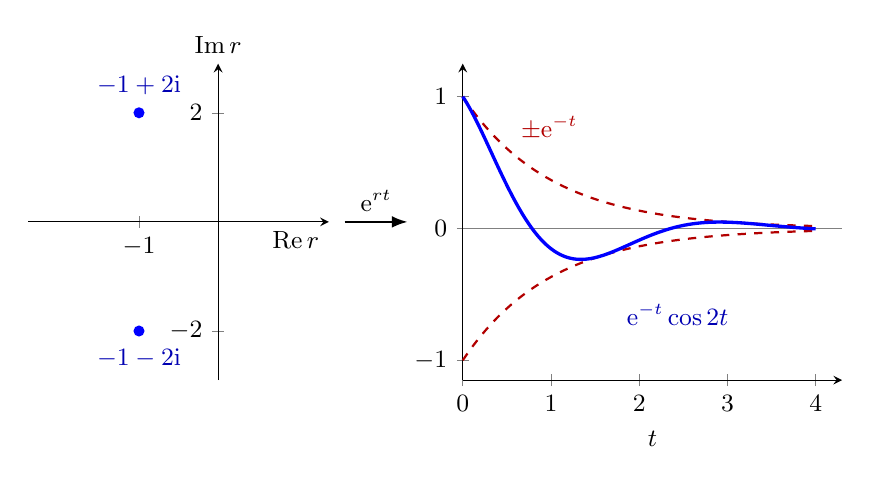
\begin{tikzpicture}[font=\small, >={Latex[length=2mm]}]
  \begin{axis}[
    name=roots, axis lines=middle, width=5.4cm, height=5.6cm,
    xmin=-2.4, xmax=1.4, ymin=-2.9, ymax=2.9,
    xtick={-1}, ytick={-2,2}, xlabel={$\operatorname{Re} r$}, ylabel={$\operatorname{Im} r$},
    xlabel style={anchor=north east}, ylabel style={anchor=south},
    clip=false
    ]
    \fill[blue] (axis cs:-1,2) circle (2pt);
    \fill[blue] (axis cs:-1,-2) circle (2pt);
    \node[blue!70!black, anchor=south] at (axis cs:-1,2.15) {$-1+2\mathrm{i}$};
    \node[blue!70!black, anchor=north] at (axis cs:-1,-2.15) {$-1-2\mathrm{i}$};
  \end{axis}
  \begin{axis}[
    at={(roots.east)}, anchor=west, xshift=1.7cm,
    axis lines=left, width=6.4cm, height=5.6cm,
    xmin=0, xmax=4.3, ymin=-1.15, ymax=1.25, xtick={0,1,2,3,4}, ytick={-1,0,1},
    xlabel={$t$}, clip=false, samples=160
    ]
    \draw[gray, thin] (axis cs:0,0) -- (axis cs:4.3,0);
    \addplot[red!70!black, thick, dashed, domain=0:4] {exp(-x)};
    \addplot[red!70!black, thick, dashed, domain=0:4] {-exp(-x)};
    \addplot[blue, very thick, domain=0:4] {exp(-x)*cos(deg(2*x))};
    \node[red!70!black, anchor=south west] at (axis cs:0.55,0.6) {$\pm \mathrm{e}^{-t}$};
    \node[blue!70!black, anchor=north west] at (axis cs:1.75,-0.5) {$\mathrm{e}^{-t}\cos 2t$};
  \end{axis}
  \draw[->, thick] ([xshift=0.2cm]roots.east) -- ++(0.8,0)
    node[midway, above] {$\mathrm{e}^{rt}$};
\end{tikzpicture}
\end{document}
